\section{Introducción} \label{sec:introduccion}

La locomoción con patas constituye una de las líneas de mayor interés dentro de la robótica móvil, principalmente por su capacidad para desplazarse sobre superficies irregulares, salvar obstáculos discretos y mantener la estabilidad en escenarios donde las plataformas con ruedas presentan limitaciones significativas \cite{siciliano2016springer}. En particular, los robots hexápodos (una configuración de seis patas) ofrecen una combinación especialmente atractiva de estabilidad estática, redundancia de apoyos y versatilidad cinemática, por lo que son idóneos para la investigación, la docencia y la experimentación.

\begin{wrapfigure}{r}{0.37\textwidth}
    \centering
    \vspace{-0.9\baselineskip}
    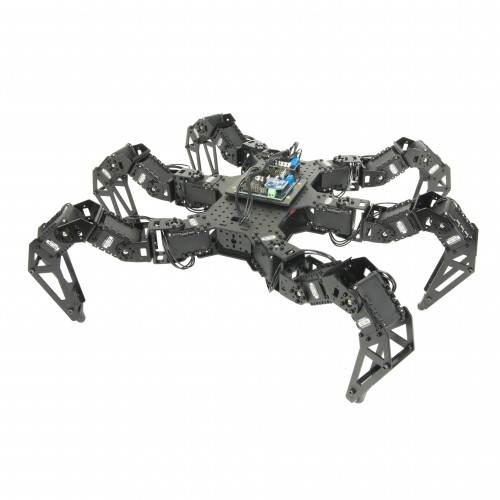
\includegraphics[width=\linewidth]{img/hexa_intro.jpg}
    \captionsetup{justification=centering,singlelinecheck=false,skip=2pt}
    \caption[PhantomX Mark III]{\centering PhantomX Mark III.\\[-2pt]{\footnotesize Fuente: elaboración propia.}}
    \label{fig:phantomx}
    \vspace{-0.8\baselineskip}
\end{wrapfigure}

Aprovechar esta capacidad exige, sin embargo, resolver problemas de control que abarcan distintos niveles de abstracción dentro de la robótica. Por un lado, la locomoción coordinada requiere modelos precisos, tanto de cinemática directa como inversa, así como la generación de trayectorias suaves y una ejecución determinista en tiempo real. Además, la operación dentro de un ecosistema robótico demanda mecanismos de comunicación, estimación de estado y compatibilidad con plataformas como ROS~2 \cite{ros2_docs}. Por este motivo, además de la estructura mecánica y los materiales empleados, la calidad de la arquitectura de control y la integración de software resultan fundamentales para el rendimiento global de la plataforma.

En este contexto, este Trabajo Fin de Grado (TFG) toma como punto de partida el kit \textit{PhantomX Mark III} de Trossen Robotics (Figura~\ref{fig:phantomx}), un robot hexápodo con dieciocho grados de libertad y estructura de aluminio, cuyo sistema original se basaba en una tarjeta ArbotiX~\cite{arbotix_controller} y en un firmware heredado de la librería Nuke \cite{nuke_hexapod}. Aunque esta solución proporciona una base funcional para el control básico del robot, presenta limitaciones relevantes en cómputo, modularidad del software e integración con herramientas actuales.

Para superar estas limitaciones en este TFG, se aborda la modernización integral de la plataforma mediante la sustitución del controlador por un microcontrolador ESP32, el rediseño de la electrónica de interfaz para el bus de comunicación con los motores y la reestructuración completa de la arquitectura software. Sobre esta base se desarrolla un motor cinemático y de marcha ejecutable en tiempo real, y se sientan las bases para su integración con una Raspberry~Pi y el ecosistema ROS~2. De esta manera, se consigue una plataforma experimental que permite la investigación y el desarrollo de algoritmos de control, navegación y planificación de trayectorias en trabajos futuros.


\section{Objetivos} \label{sec:objetivos}

De acuerdo con lo anterior, el objetivo general de este trabajo es modernizar la plataforma \textit{PhantomX Mark III} para dotarla de una arquitectura hardware-software modular, capaz de ejecutar locomoción en tiempo real e integrarse con ROS~2, dejando preparada la plataforma para futuras capacidades de navegación.

\begin{enumerate}

    \item \textbf{Rediseñar la capa de control de actuadores:} desarrollar el driver de bajo nivel para los servomotores DYNAMIXEL AX-12A sobre bus serie \textit{half-duplex}, junto con la electrónica de adaptación y el diseño de la placa de circuito impreso (PCB).

    \item \textbf{Formalizar el modelo cinemático del robot:} definir la cinemática inversa de cada extremidad e implementar el conjunto de transformaciones que relacionan las patas, el cuerpo y el sistema de referencia global.

    \item \textbf{Implementar el motor de locomoción:} diseñar los algoritmos de coordinación de marcha y generación de trayectorias necesarios para su ejecución determinista en tiempo real sobre el microcontrolador.

    \item \textbf{Integrar la plataforma en el ecosistema ROS~2:} establecer la comunicación entre el ESP32 y una Raspberry~Pi, de forma que el robot pueda intercambiar comandos, estado y odometría con nodos del ecosistema ROS~2.

\end{enumerate}

\section{Estructura del documento} \label{sec:estructura_memoria}

Con la intención de ofrecer una visión organizada de la memoria, se ha adoptado una estructura que progresa desde los fundamentos matemáticos necesarios para comprender la locomoción de la plataforma hasta las decisiones de diseño e implementación que concretan el proyecto. En consecuencia, el documento se estructura de la siguiente manera:

\begin{itemize}
    \item \textbf{Capítulo 2, Estado del arte:} repasa el contexto y los trabajos previos en robots hexápodos y en el control de plataformas multípedas.

    \item \textbf{Capítulo 3, Marco teórico:} desarrolla la cinemática, las transformaciones y las estrategias de marcha en las que se apoya el motor de locomoción.

    \item \textbf{Capítulo 4, Plataforma hardware e implementación:} describe la electrónica, el software y la integración con ROS~2 desarrollados en el proyecto.

    \item \textbf{Capítulo 5, Validación, conclusiones y líneas futuras:} recoge las pruebas realizadas sobre el sistema, valora el cumplimiento de los objetivos y las limitaciones encontradas, y propone las posibles líneas de trabajo futuro.
\end{itemize}
